
\chapter{Introduction}
The field of statistics has undergone fundamental changes in the past
twenty years as computers have made significant gains in memory,
processing speed, and storage capacity: we can now collect ever
greater quantities and varieties of data and analyze these data with
complex, computationally intensive methods.  As a result, it is
increasingly important for statisticians to have basic skills and
literacy in data technologies.  In this book we examine how
statisticians use the computer expressively to analyze data.  Our
approach blends modern statistical methods with the computational
aspects of acquiring, analyzing, and reporting data.

The emphasis here is on the statistical thought process in the context
of computing with data.  We use case studies to highlight some of the
exciting research currently being done in the field of statistics as
well as to exemplify the interplay between scientific context,
statistical concepts and computation.  In these real-world
applications we see how statistical concepts guide our investigations
and how these investigations rely fundamentally on our abilities to
interface with data in a technological context.

While our focus will be on data and data technologies, we will also
explore statistical techniques that have emerged because of the
improved performance of the computer.  Techniques such as
cross-validation, the bootstrap and classification trees are examples of
methodology that exist in statistical practice only because computing
is so ubiquitous and powerful.  These techniques give us much more
flexibility when analyzing data.

In addition to new statistical methodology, the computer provides us
with an auxiliary tool for statistical investigations that complements
mathematical understanding.  Simulation allows us to explore
existing methodologies in a ``hands on'', practical manner in order  to
understand their characteristics.  We can generate numerous samples
under different contexts and see how different methodologies
perform.  And we can investigate hypotheses about potential new
methodologies before we attempt to understand them mathematically.
This two-fold approach of mathematics and simulation can be very
empowering as it gives alternative ways to explore and understand
statistical concepts.

Before we proceed, we should point out that while this book is about
computing, the goal is to provide a solid basis for the fledgling
statistician so that she can make good use of the computer to
understand statistical concepts and approach data analysis with
confidence.  For this reason, the focus here is on data analysis and
answering scientific questions, rather than on computing for its own
sake. The view here is of computing as a tool, complimentary to
mathematics tools, that leads to our main goal: to better understand data and
statistical concepts and to improve our contributions to  answering scientific
questions.


\section{Data} 
% Taken from Mark's summer.stat.ucla.edu website
Today, almost every aspect of our lives is rendered in data.  New data
collection technologies have made it easy to record continuous,
high-resolution measurements of our physical environment (weather
patterns, seismic events, the human genome). We're also constantly
monitoring our movements through and interactions with our physical
surroundings (automobile and air traffic, large-scale land use,
advanced manufacturing facilities). In computer-mediated settings, our
activities either depend crucially on or consist entirely of complex
digital data (networked games, peer-to-peer technologies, Web site and
Internet usage).  As a reflection of the diversity and variety of the
``systems'' under study, these data-based descriptions of our world
tend to be massive in size, dynamic in character, and replete with
rich structures.    That is, the data available often depart from  the traditional 
notion simple rectangular arrays of numbers.  Simple alternatives to
the matrix or numbers  are data as ragged arrays of numeric measurements, 
free-formatted text, or images and video.  We describe a few examples 
where such data arise.    


\subsection{Rainfall: Numeric data with many missing values}

Whether rainfall comes in a limited series of intense events or is
more evenly distributed over many days impacts how land and roadways
are developed for agricultural, industrial, and social purposes.  The
flooding of New Orleans in 2005 from Hurricane Katrina and the
resulting breaks in the levee system offers one devastating example.
Meteorological data, and, in particular, precipitation data, help us
develop dam specifications and plan for floods in urban areas.  The
study of precipitation also plays an important role in the study of
global warming because changes in the level of precipitation can have
a large economic and ecological impact.


Extreme weather events are by their nature rare events that we do not
have the opportunity to observe many times, but nonetheless we need to
prepare for them.  For example, scientists are faced with the problem
of determining an extreme rainfall event that may happen once in a
hundred years from only fifty years of data.  At the U.S. National
Center for Atmospheric Research, meteorologists, earth and planetary
scientists, and statisticians analyze rainfall data to better predict
these extreme rainfall events.  An example of the data that these
scientists use in making their predictions is the daily precipitation
records measured in a network of 56 weather stations in the Colorado
Front Range.\footnote{These data  have been made
 available to us by Doug Nychka, National Center for Atmospheric
  Research.}  Altogether there are about 400,000 measurements observed
in this network, with the earliest recordings dating back to 1948.
However, these data do not make up a neat rectangular array of numbers
because while some weather stations have been in regular operation
since 1948, others are no longer in operation, and many others are
only been collecting data for about 30 years.

A snippet of the data is presented in Figure~\ref{fig:rainData}, where
the daily precipitation is reported in hundredths of an inch, i.e.\
112 denotes 1.12 inches of rain in a 24 hour period.
Figure~\ref{fig:rainMissing} gives a visual display of the times that
the weather stations were in operation.  Each row of dashes in the
figure corresponds to one weather station, and the gaps between the
dashes denote the times when the station was not recording rainfall.
The regularly patterned vertical white strips correspond to the winter
months, i.e. when precipitation is in the form of snow rather than
rain. This figure helps show the structure of the data; in particular
it is easy to see that there are many missing values due to the
varying operating periods of the stations.


\begin{table}
{\footnotesize
\begin{verbatim}
  [1]   0  10  11   1   0   0   0   0   0   0   0   0  10   0   0   0   0   0
 [19]   0   0   0   7  18   0   0   0   0   0   0   0   0   0   0   0   0   0
 [37]   4  15   0   0   0   0   0   0   0   0   0   0   0   3   0   0   0   0
 [55]   0   0   0  45   0   3  28   0   0   0   0  41   2   0   0   0   0   3
 [73]   0   0   0   0 112   0   0   0   0   0   0   0   0   0   0   0   9   2
 [91]   0   0   2  18   0   0   0   0   0   8   7   3   0   0  14  53   0   0
[109]   0   0   0  10   0   0   0   0   0  63   5   0   0   6   0   0   0   0
[127]  66  76   5  13   2   2 103   8  25   0   1   2   0   0   0   0   0   0
[145]   0   0   0   0   4   0   0   0   0   4   6  90 257   2 159   6  18  30
[163]  55   5  33  16   1   0   0   0   0   0   0   0   0   0   0   1  11   4
[181]   0   0   0   0   0  18  22  31  16  25  42   0   2   9   0   0   0  19
[199]   0   0  16   0   0   0   0   0  30   0   0   0   0   0   0   0   0   0
[217]   9   0   9   0   0  25  32   1   9   5   0   0   0   0   4   0   0   0
\end{verbatim}
}
\caption{A few observations from daily rainfall, measured in 
  hundredths of an inch (e.g. 103 represents 1.03 inches), 
  on 9,838 days from 1948 to 2002 at one of the 56 weather stations 
  in the Colorado Front Range.  A zero indicates no rainfall for that
  day, whereas a day when the weather station is not in operation is left 
  out of the array of values.}
\label{fig:rainData}
\end{table}

\begin{center}
\begin{figure}
 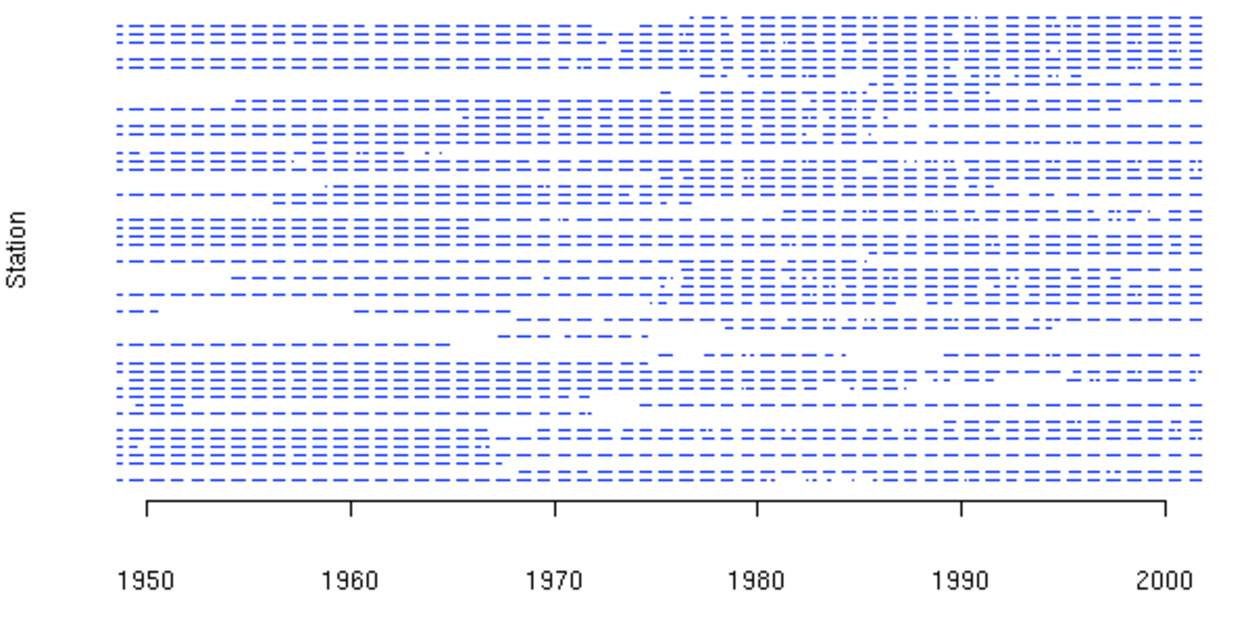
\includegraphics[width=5.5in]{Introduction/images/rainImg/operatingStations.pdf}
 \caption{Each row in this strip chart correspond to one of the 56
   weather stations in the Colorado Front Range. Blue indicates the
   days when the station was in operation, and white represents the
   days when it was not in from 1948 to 2002.  We see that some
   stations have been regularly recording rainfall since 1948, others
   have only been in operation since the mid 1970s, and still others
   have been in and out of operation over this fifty-year period.  The
   regularly spaced vertical white stripes correspond to the winter
   months when rainfall is not recorded.}
\label{fig:rainMissing}
\end{figure}
\end{center}


In addition to the precipitation values for each day, the NCAR
scientists use other information about the weather stations in their
work such as the location of the weather station, i.e.\ latitude,
longitude and elevation.

With these data, scientists examine the distribution of large
precipitation events and how this distribution may vary over
geographic location.  These are first steps toward answering important
questions such as how to assess the ability of computer climate models
to predict rainfall when they have to extrapolate irregularly located
station observations and many missing observations.  To address these
questions, statisticians use modern statistical mapping techniques and
surface fitting techniques, such as thin plate splines, in their
analyses of the rainfall data.

\subsection{Spam: Free-formatted text as data}
Well over half of the electronic email messages moving through the
Internet are ``spam'', unsolicited bulk electronic mailings.  These
unwanted messages are often offensive to read and it can be time
consuming and aggravating to sort through your inbox to delete them.
To reduce the amount of unwanted electronic mail in your inbox,
Internet providers deploy automatic spam filters (software) to
separate spam from regular email communications before it reaches a
client's inbox.  These filters need to determine whether or not an
email message is spam according to various characteristics of the
message.  Statisticians and computer scientists have had some success
with this prediction problem by using modern statistical techniques
such as Naive Bayes estimation and artificial neural networks.  For
example, Spam Assassin, a company which has developed a filter which
they describe as an
\begin{quote}
  intelligent email filter which uses a diverse range of tests to
  identify unsolicited bulk email, more commonly known as Spam.  These
  tests are applied to email headers and content to classify email
  using advanced statistical methods \textit{including a Bayesian
    statistical learning component}...
\end{quote}
Spam Assassin's email filter took top honors in 2005 in the Anti-Spam
category of Datamation's Product of the Year for their email filter,


\begin{figure}
{\footnotesize
\begin{verbatim}
Return-Path: whisper@oz.net
Delivery-Date: Fri Sep  6 20:53:36 2002
From: whisper@oz.net (David LeBlanc)
Date: Fri, 6 Sep 2002 12:53:36 -0700
Subject: [Spambayes] Deployment
In-Reply-To: <LNBBLJKPBEHFEDALKOLCIEJABCAB.tim.one@comcast.net>
Message-ID: <GCEDKONBLEFPPADDJCOECEHJENAA.whisper@oz.net>

You missed the part that said that spam is kept in the "eThunk" and was
viewable by a simple viewer for final disposition?

Of course, with Outbloat, you could fire up PythonWin and stuff the spam
into the Junk Email folder... but then you loose the ability to retrain on
the user classified ham/spam.

David LeBlanc
Seattle, WA USA

> -----Original Message-----
> From: spambayes-bounces+whisper=oz.net@python.org
> [mailto:spambayes-bounces+whisper=oz.net@python.org]On Behalf Of Tim
> Peters
> Sent: Friday, September 06, 2002 12:24
> To: spambayes@python.org
> Subject: RE: [Spambayes] Deployment
>
> [Guido]
> > ...
> > - A program that acts both as a pop client and a pop server.  You
> >   configure it by telling it about your real pop servers.  You then
> >   point your mail reader to the pop server at localhost.  When it
> >   receives a connection, it connects to the remote pop servers, reads
> >   your mail, and gives you only the non-spam.
>
> FYI, I'll never trust such a scheme:  I have no tolerance for false
> positives, and indeed do nothing to try to block spam on any of my email
> accounts now for that reason.  Deliver all suspected spam to a Spam folder
> instead and I'd love it.
> _______________________________________________
\end{verbatim}
}
\caption{An example of an e-mail message from the set of approximately
  9,000 classified messages provided by Spam Assassin for testing new
  statistical techniques and algorithms for filtering email. This
  particular mail message is not Spam.}
\label{fig:sampleEmail}
\end{figure}


To develop filtering algorithms, test cases are needed where the
electronic mail messages have been manually classified as spam or ham
(regular mail).  The collection of mail messages is used to see how
well a filter does at identifying spam as spam and ham as ham.
Spam Assassin\\
\texttt{http://spamassassin.apache.org/} has classified and made
publicly available over 9,000 mail messages, of which about 2,500 are
spam.  One of these messages appears in Figure~\ref{fig:sampleEmail}.
Spam Assassin provides each mail message in a plain text file that
includes the header, body and any attachments in the email. These
emails are organized into separate directories for spam and ham
messages.  Although these messages do not conform to our typical sense
of scientific data, they make the basis for test data required to
validate the performance of filtering algorithms.

To develop and test models and rules for predicting spam, we convert
these text messages into a format that would facilitate in-depth
statistical analysis.  For example, we might examine the body of a
mail message and record how many occurrences of various words (or even
all possible words) appear in the message.  Additionally, we might
derive variables that measure certain characteristics of the message,
such as the use of exclamation marks in the subject line, capitals in
the body of the message, and the time of day the message was sent or
received.  The task of determining which variables to create also
requires statistical investigation.  Modern statistical classification
methods have proven quite successful in all of these endeavors.

\subsection{Search and rescue: Satellite images}
On the morning of January 28, 2007, Jim Gray set sail, heading out San
Francisco's Golden Gate to the Farallon Islands, a wildlife refuge 27
miles offshore. Gray was last seen that afternoon a mile or two from
the Farallons by a naturalist who was on one of the islands, then he
disappeared.

In an article written by Steve Silberman about Gray's disappearance,
Silberman describes Gray as a ``computing legend'' whose
\begin{quote}
  work helped make possible such mainstays of modern life as cash
  machines, ecommerce, online ticketing, and deep databases like
  Google.  ``Jim's work inspired us and many other computer scientists
  to seek out and tackle very ambitious projects,'' says Google
  cofounder Sergey Brin. ``He never shied away from problems involving
  large-scale data and computation.''
  ...\\
  The notion of searching for Gray with tools he helped invent struck
  a deep chord in the online world.
\end{quote}

Friends and collaborators of Gray's got to work searching for signs of
his boat, called the Tenacious, in satellite images taken a few days
after his disappearance.  The Canadian Space Agency flew the
Radarsat-1 satellite over the area taking pictures with radar.  Then
Digital Globe's QuickBird and GeoEye's Ikonos satellites made several
passes over the San Francisco Coastline.  NASA had one of its ER-2
planes fly about 20 kilometers above the ocean taking pictures with
its near-infrared camera.  All together hundreds of gigabytes of image
data were collected.

For example, each image from the ER-2 was $4072 \times 4072$
pixels. Collaborators of Gray's at Johns Hopkins used the computer to
break up these images into smaller tiles and look for the Tenacious,
which would only be a few pixels large.  They used statistical
techniques to search the images for clusters of a few pixels with high
intensities, possibly denoting the white boat, but not too many
clusters, as that probably denoted clouds. Likely images were then
reviewed by eye to confirm whether there was something in the image
that could potentially be a sailboat.  Figure~\ref{fig:tenacious}
shows one of the tiles found through this computer vision approach.

\begin{figure}
 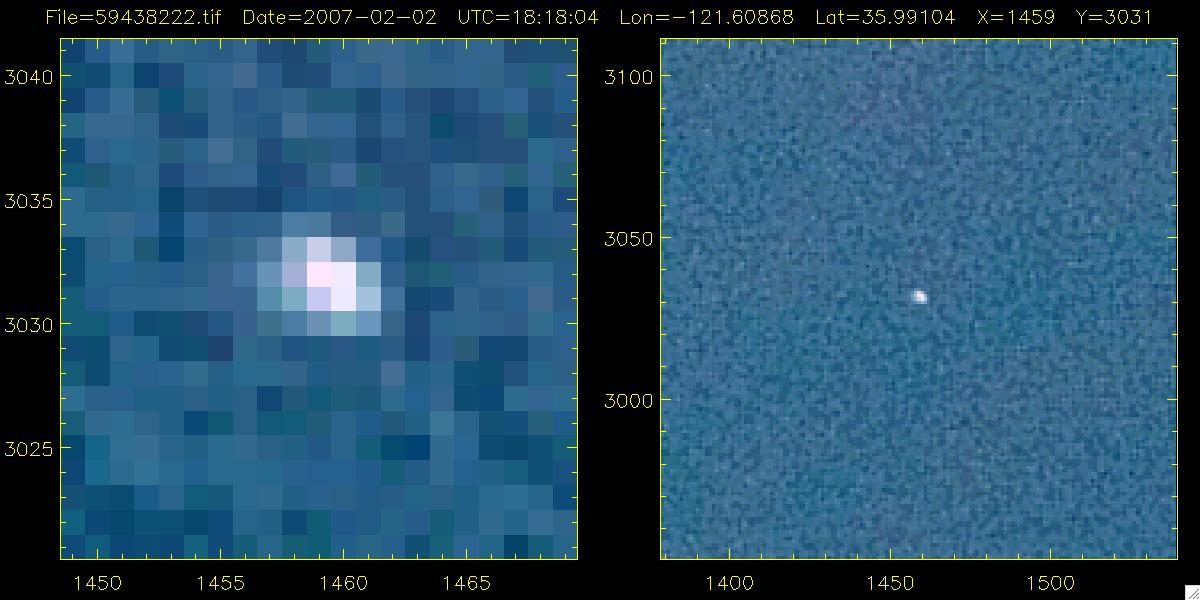
\includegraphics[width=6in]{Introduction/images/tenacious/ER-2.jpg}
  \caption{ (\url{http://skydev.pha.jhu.edu/nieto/Tenacious/images/ER-2/})}
\label{fig:tenacious}
\end{figure}

The search was particularly difficult due to the cloud cover, white
caps, wakes, and other whitish blotches on the mostly gray images.
Given the difficulty of finding ``interesting objects'' using the
computer's ``eyes'', a second effort was mounted by another
collaborator of Gray's to search through the images.  This effort, led
by a scientist at Amazon, used human eyes, or ``artificial artificial
intelligence''.  Amazon's service, called Mechanical Turk, organized
thousands of volunteers to sift through hundreds of thousands of
images looking for any sign of the Tenacious.

The Coast Guard pledged to follow any lead that any group turned up.
Several images looked promising, and ocean modelers at NASA's Jet
Propulsion Lab (also associates of Gray's) used data from Coast Guard
buoys to predict where the boat might have drifted from the time that
the pictures were taken.  Unfortunately, despite these amazing
efforts, the Tenacious was not found. Although the search failed, it
is widely recognized that these new data analysis tools that use
remote sensing images for search and rescue efforts have great
potential.


\begin{comment}
\subsection{Traffic: Video}

\begin{figure}
  \begin{tabular}{cc}
 \includegraphics[angle=90,width=3in]{Introduction/images/trafficImg/aViewfromCamera6.png}
&
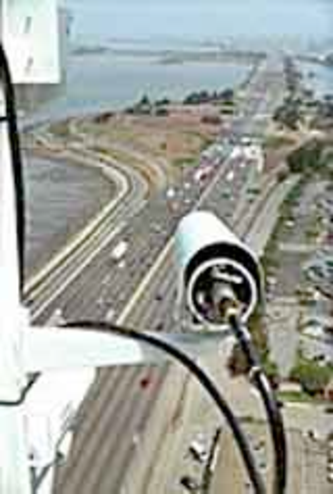
\includegraphics{Introduction/images/trafficImg/videoCam.pdf}
  \end{tabular}
  \caption{The Berkeley Highway Laboratory is a 2.7 mile section of
    Interstate 80 that's observable with a bank of twelve video
    cameras on the roof of Pacific Park Plaza, a 30-story building
    beside the freeway. The video frame from the camera shown here is
    looking north; the field of view is furthest down the freeway.  It
    covers the longest stretch (about one mile) from the Ashby Avenue
    on-ramp to University Avenue
    off-ramp. (\texttt{http://www.stat.berkeley.edu/users/fspe/I80/movie2-new.mpg})}
\label{fig:videoCam}
\end{figure}

\begin{figure}
  \begin{center}
   \leavevmode
 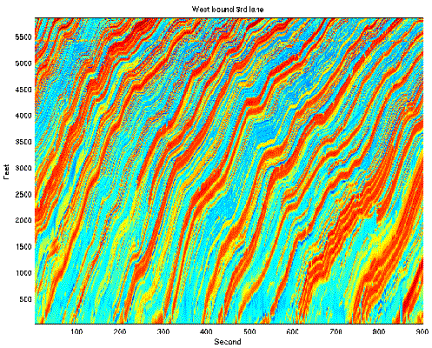
\includegraphics[width=5.5in]{Introduction/images/trafficImg/westboundLane3.png}     
\caption{A multi-colored intensity profile for a short section of 
Interstate 80 over a 15 minute time period.  (Rice and Cho \texttt{http://www.stat.berkeley.edu/users/fspe/I80/I80.htm})}
\label{fig:intensityProfile}
  \end{center}
\end{figure}


Some one about to travel on the California freeway system typically
wants to know how long it will take to arrive at their destination
and which alternate routes would be the fastest.
Transportation engineers and statisticians use a network of 
$22,000$ loop detectors located throughout the freeway system to
monitor traffic and develop such predictions. 
These detectors are embedded in the road surface and 
provide information such as the number of cars crossing over the
detector every 30 seconds, which amounts to 2GB of information 
collected a day.  
Using past traffic patterns and current condition as supplied by these 
detectors, statisticians fit models to predict the fastest route
from one location to another.


To improve the quality of the predictions, scientists are now exploring
the use of video cameras to complement existing loop detectors. 
The Berkeley Highway Laboratory has mounted video cameras on top of buildings
near a section of Interstate 80 to monitor traffic on the freeway
(see Figure~\ref{fig:videoCam}).

These video data have the advantage over loop detectors in that they
are easy to maintain and they provide better spatial coverage.
However, they present real challenges related to computer vision,
i.e.\ how can computers ``see'' the cars on the freeway in the video
recordings?  Statisticians have developed techniques based on the
behavior of stochastic processes to convert these low-resolution
images into information about traffic intensity across time and space.
For example, the multi-colored intensity profile in
Figure~\ref{fig:intensityProfile} describes the aggregate behavior of
vehicles in a stretch of the middle lane of the westbound traffic over
a brief fifteen minute time period. With this information in hand,
algorithms can be developed and tested that pull out useful
information such as the speed of traffic at a particular location.
\end{comment}

\section{The  Data Analysis Process}
None of the data in the examples of  the previous section come in
a traditional row-column format that is ready for statistical
analysis.  The missing recordings of rainfall need to be carefully
investigated before proceeding with a more in-depth analysis of the
distribution of extreme weather events.  The email messages require a
lot of processing in order to extract useful information for
developing a prediction procedure, and the cloud cover and temporal
nature of the images needs to be considered when searching
for small, high-intensity clusters.  Most
statistics texts limit their exposition of data analysis to examples
where data have already been distilled into a rectangular table of
numbers that are prepared for the application of a particular
statistical method.  To use common statistical methods, we may end up
projecting the raw data into a rectangular array of numeric values.
However, the process of figuring out how to create these variables
from raw input is an important part of the data analysis process.  Our
goal here is to bring to the forefront this entire process, which
includes the need to be able to acquire, clean, and summarize data,
as well as to model and validate the model with data, and to 
report findings from the analysis.

Handling raw data is both interesting and non-trivial.  It requires a
facility with data analysis and also the ability to express
computations that help readily explore the many different ways to
reduce the information into a format for further, deeper analysis.
Curtailing the data analysis process in this way can greatly impact a
statistician's ability to do interesting, high-qualilty analysis.
That is, not being able to work directly with the raw data limits a
scientist greatly.  Analyzing data requires knowledge about the
particular topic being studied and of appropriate statistical methods,
and it also requires the ability to be able to apply those methods to
the relevant data.  This includes accessing the data values,
transforming them into the appropriate form, applying statistical
methods to the data and exploring the results.  Computing and data
technologies are as essential for data analysis as understanding what
statistical methods are appropriate for the data.  Computation is the
vehicle by which we move data into information.

One must be able to access data in different forms, examine them to
see what one has, find relevant subsets, model them or find the
``signal'' and iterate these steps and ultimately report ones
findings.  This iterative cycle of data analysis requires facility
with one or more computer languages so that expressing the
computations fades into the background and becomes a means to an
end. It should not be a hurdle that diverts one from the data analysis
task and scientific question.  For this to be true, one must take
learning computing seriously and try to understand it rather than
simply parrot examples. A good understanding of these fundamental
ideas and concepts will be of immense value to you in whatever field
you pursue as it will surely involve decision making, data and
computation.


Even when our focus is not on a particular scientific problem or set
of data, but rather in understanding characteristics of mathematical
or statistical methodology itself, the computer is a terrific new tool
at our disposal.  In the past, we relied almost exclusively on
mathematical techniques to explore a particular method and how it
would behave under different circumstances.  When doing research, we
might have attempted to prove a mathematical result without really
knowing if it were true or not.  We can now use the computer to
simulate the behavior of a method to gain a better understanding and
to gain intuition about its behavior.  With intelligent experimental
design, we can vary the inputs to a simulation to more efficiently
understand the different characteristics of a computational approach.
And the computer therefore serves as an additional tool along with the
more traditional mathematical approach.  And these two serve as
complementary media for describing and discussing scientific research.



\begin{comment}
\section{Overview of material covered}

As we mentioned above, we will discuss the different stages in the
data analysis cycle from start to end.  We won't emphasize the
statistical methodology, but we will introduce both general
computational techniques such as the bootstrap and cross
validation. Also, we will make use of methodology that you may not
have seen in other statistics classes and we will provide a brief,
heuristic introduction to each of these.

We focus on scientific questions and how we might acquire, summarize,
clean, model and report the data and results.  This is not about
applying statistical methods to example data. Rather the question
tells us what statistical techniques might be relevant and
appropriate. Some of these are complex and some are simple. We prefer
the simple approach if it is adequate and in keeping with the
scientific question and the accuracy and precision needed in the
answer.  Please don't use statistical techniques that are not
appropriate or overkill for the task at hand. Start by looking at the
data and producing interesting, meaningful graphical summaries.  Well
composed (the thinking process) and created (via software) plots are
often the most compelling answers.  Blind use of linear models tend to
be superficial and associated with a mechanized response rather than
an understanding of the particular data.

These examples all have a similar structure when it comes to answering
a question with data --

     \begin{itemize}
     \item Data ACQUISITION --- Input/output, regular expressions 
     \item Data CLEANING, verification, and manipulation --- graphics, exploratory data analysis
     \item Data ORGANIZATION --- data frames, XML, databases
     \item MODEL the data --- fit statistical models to the data 
     \item Data as a PSEUDO-POPULATION --- assess the fit of the model via the
     bootstrap, cross-validation 
     \item SIMULATED data --- simulation studies 
     \end{itemize}

In this cycle we encounter: 
\begin{itemize}
\item Statistical Concepts
\item Computing Concepts
\item Software
\end{itemize}

These three concepts will be interwoven throughout 
the text. 

In the book, we will look at various data and computing technologies.
These include
\begin{itemize}
\item the R statistical computing language and environment;
\item simulation and random number generation;
\item bootstrapping for estimation, and cross valdation for model selection;
\item processing text with pattern matching via regular expressions;
\item simple data manipulation and analysis using shell tools;
\item parsing structured data in the form of XML --- the eXtensible Markup Language;
\item accessing remote, structured data in relational database
  management systems via the client-server model of computing
and SQL --- the Structured Query Language.
\end{itemize}
This involves at least five different languages.
We could explore other languages such as Perl
and Python, but we won't as we can do most things using
R and the shell tools.  But one should be aware of these
other languages and tools.

We will also cover aspects of visualization, both the basic aspects of
using R to produce plots and also how to think about what plots to
create.  And we will encounter some non-classical, even modern,
statistical methods such as classification and regression trees, k-th
nearest neighbor classification, Bayesian models, thin plate splines
(TSP).



\subsection{Statistical Concepts}

\begin{itemize}
\item Graphics
        \begin{itemize}
        \item elements of graphing data
        \item grammar of graphics
        \item advanced plotting
        \end{itemize}

\item Computationally intensive methods
        \begin{itemize}
        \item Classification and Regression Trees
        \item Kth Nearest Neighbor clustering
        \item Thin plate splines 
        \end{itemize}

\item Simulation tools 
        \begin{itemize}
        \item Bootstrap
        \item Cross-validation
        \item Monte Carlo Markov Chain 
        \end{itemize}
\end{itemize}

\subsection{Computing Concepts}

\begin{itemize}
\item Programming concepts - e.g. loops, recursion, trees

\item Regular expressions and text manipulation

\item Relational Databases

\item Random number generation

% \item Representation of numbers in the computer 

% \item Event handling and GUI development
\end{itemize}

\subsection{Software}

\begin{itemize}
\item R - statistical software
\item Unix - shell commands
\item Regular expressions
% \item Perl 
\item SQL - Structured Query Language for relational databases 
\item XML - Extensible Markup language
% \item Gtk - GNU Toolkit for creating graphical user interfaces
\end{itemize}

\end{comment}

\begin{comment}
\section{Goals of the Course}
\begin{itemize}
\item
  Focus:  use existing software and functionality
   for context-specific analyses.
\item
  Learn about: box of tools and how to use them
   to create things, and even build new tools.
   \\
   Learn about currently emerging technologies
\item
   De-emphasize: understanding the existing algorithms.
  \\
     Be able to intelligently discuss different 
     technologies and tools, knowing when to use them and what are
     the trade-offs

\item
    Understanding fundamental algorithms is important 
    if you need to
\begin{itemize}
\item
    recreate them in a new language
\item
    use them in new ways when developing new algorithms.
\end{itemize}

\item Practical: how statistical methodology is used
    in Industry, Laboratory, Research 

\item
  Focus: overall task not just on the application of 
  specific statistical methodology but on 
  how to think about approaching problems related to
  computing on data
\end{itemize}

 

\begin{itemize}
\item
  How to think about approaching problems related to
          computing on data
\item
  Learn about currently emerging technologies
\item
  Be able to intelligently discuss different 
     technologies and tools, knowing when to use them and what are
     the trade-offs
\item
  Be able to find out about and learn other technologies
\end{itemize}
\end{comment}

